\chapter{Binned and bin-free analysis of Fluorescence Enhancement by gold nanorod on a 2D layer}
\label{chapter:binfree}
\graphicspath{{./chapters/c3_binfree/figures/}}
%============================ MAIN ================================

\begin{abstract}
Gold nanorods are extensively used for single-molecule fluorescence enhancement as they are easy to synthesize, bio-compatible and provide high light confinement at their nanometer-sized tips. The current way to estimate fluorescence enhancement relies on binned time traces or on fluorescence correlation spectroscopy (FCS). We report on novel ways to extract the enhancement factor in a single-molecule enhancement experiment, avoiding the arbitrary selection of one or a few high-intensity burst(s). These new estimates for the enhancement factor make use of the whole distribution of intensity bursts, or of the interphoton delay distribution, which avoids the arbitrary binning of the fluorescence intensity time traces. We present experimental results on the bi-dimensional case, experimentally achieved using a lipid bilayer to support the diffusion of fluorophores.  We support our findings with histograms of fluorescence bursts and with an analytical derivation of the interphoton delay distribution of (nearly) immobilized emitters from the fluorescence intensity profile.
\end{abstract}
\newpage
%============================ Introduction =====================================
\section{Introduction}
Single quantum emitters such as fluorophores, quantum dots, color centers 
and fluorescent proteins have become powerful tools for modern science 
since they provide nanometer-sized probes that can be used to extract 
information about the local environment \cite{moerner1999illuminating, kulzer2010single}, 
oxidation state of molecules \cite{zhang2017gold} and proximity of other 
emitters using F\"oster resonance energy transfer (FRET) \cite{jares2003fret,stein2011single,kalinin2012toolkit}. 
These unique advantages are joined to those of non-invasive optical methods. 

%-Fluorescence enhancement by plasmonic structures paragraph: physical origins, dependence, mention emission and excitation. limitations. motivate the quantification of enhancement in different structures.
Fluorescence enhancement by plasmonic nanostructures has been successfully 
used in the past to increase the signal from weak 
emitters \cite{kinkhabwala2009large, yuan2013thousandfold, khatua2014resonant} even in 
living cells \cite{vanzanten2010imaging}. In a nutshell, fluorescence enhancement
by metallic nanoparticles refers to a considerable increase in the rate of detected 
photons whenever a (often weakly) fluorescent molecule is placed in the vicinity of the nanoparticle.
Enhancement heavily relies on the surface plasmon resonance of the nanoparticle, which often lies
in the optical spectral range. When excited at this resonance frequency, 
the nanoparticles can concentrate optical fields in tiny volumes,
the so-called ``hot spots'', providing a sub-diffraction 
working volume that can be exploited to extend the powerful technique fluorescence 
correlation spectroscopy (FCS) to micromolar 
concentrations \cite{estrada200810000,manzo2011nanoscale,kinkhabwala2012fluorescence,punj2013gold,khatua2014enhancedfluorescence}. 
Notably, this approach was also used to study molecular diffusion in the membrane 
of a living cell \cite{flauraud2015largescale}.
Fluorescence enhancement also provides a way to extend the powerful tools of single-molecule spectroscopy to 
weakly emitting species.


Regardless of the origin of the fluorescence photons, a usual approach is to record the arrival time of each individual 
photon in the so-called time-correlated single-photon counting (TCSPC) approach in a time-tagged 
time-resolved (TTTR) configuration  \cite{Wahl_picoquant,becker2015advanced}. 
Thanks to the high-speed electronics and pulsed excitation sources available commercially, 
the absolute arrival times (also called macrotimes) can be determined with picosecond accuracy and, with the proper synchronization to the excitation source, the ``nanotimes'' \footnote{The usual denomination is microtime but we opt for nanotime to avoid confusion with the macrotime.} can be also determined. 
The nanotime is usually used to obtain the lifetime histogram, which can be used to 
gain insight into the underlying mechanism of the emission. For example, 
in the case of fluorescence, the radiative and non-radiative rates can be accessed experimentally with a 
measurement of the lifetime if the quantum yield is known \cite{lakowicz2007principles}.
%Figure \ref{fg:tcspc} shows an time representation for such an experimental configuration. 
The output of a TTTR experiment can be represented as a classical function of time \cite{Lippitz2005}:

\begin{equation}
I(t) = \sum_i \delta( t-t_i)
\label{eq:intensity_TCSPC}
\end{equation}
where $\delta(t)$ is the usual Dirac function and $t_i$ is the absolute arrival time
for each detected photon in the experiment (measured relative to the start of the experiment, the macrotime). 
We shall call this function \textit{unbinned time trace}. 
 

 %\begin{figure}
 %\includegraphics[width=\textwidth]{img/TCSPC_scheme.pdf}%
 %\caption{\textbf{Time-correlated single-photon counting detection scheme.} Typical configuration for a time-tagged time-resolved photoluminescence experiment. The exciting source is a pulsed laser with MHz repetition rate and both the time tag $T$ since the start of the experiment and the TCSPC time $t$ are recorded and saved. The former can be used to calculate the interphoton delay distribution and the latter to generate a lifetime histogram to obtain, for example, the lifetime of a fluorescent molecule. Modified from \cite{Wahl_picoquant}.
%\label{fg:tcspc}}
 %\end{figure}

In spite of the high temporal resolution provided by such experiments, 
the usual way to characterize the emission of quantum emitters is to 
display the time trace of the number of detected photons 
in a certain integration time (or binning time) and to
complement this with a histogram of detected photon counts per time bin. 
Such a characterization inherently introduces an arbitrary parameter, 
the binning or integration time, that may bias the obtained distribution \cite{Lippitz2005}. 
Alternatively, correlation functions can be calculated from the unbinned
 time trace to exhibit the characteristic 
time of a process of interest, such as the diffusion \cite{magde1972thermodynamic,haustein2007fluorescence} 
or rotation \cite{loman2010measuring} characteristic times of molecules in solution as well as 
other molecular properties even at single-molecule level \cite{medina2002fluorescence, ghosh2017quantifying}.
This approach can provide estimates of the enhancement factor, but is very sensitive to 
background corrections \cite{pradhan2016goldnanorodenhanced, langguth2014simple}. 
The common practice to determine fluorescence enhancement is to screen the time trace 
for the strongest fluorescence burst(s), corresponding to unlikely event(s) that a 
molecule occupies the best position in the hot spot of the plasmonic near field for 
a long enough time. This procedure, often nicknamed ``cherry-picking'', depends on the 
binning time, on the diffusion constant, and on the stochastic character of each 
molecule's trajectory. There is no warranty that waiting for longer times, or binning 
at higher resolution, wouldn't lead to larger enhancement factors. Therefore, there 
is a pressing need for less arbitrary ways to quantify the enhancement factor. 

Here, we focus on the use of a less common quantity, the 
\textit{interphoton delay distribution} $p(\tau)$,
to characterize the emission of quantum emitters and to extract reliable 
information about an emitting system avoiding the introduction of any arbitrary 
binning time. The interphoton delay distribution expresses the delay distribution 
between consecutive photons: after each photon detection, the probability density to observe 
the next photon at a time $\tau$ is $p(\tau)$ ($p(\tau)\geq 0$) \cite{Verberk2003}.
Experimentally, it can be obtained by simply plotting a histogram of the time differences between 
successively detected photons.

In this paper we present a model to relate the interphoton delay distribution
to the spatial distribution of fluorescence intensity delivered by a 
single quantum emitter in the limit of \textit{slow} diffusion. We show that $p(\tau)$ 
encodes information about the intensity distribution inside the volume accessible 
to diffuser. We will illustrate this point with single-molecule fluorescence 
in a bi-dimensional case both with a Gaussian beam shape and with addition of a power-law model of 
enhanced fluorescence by a gold nanorod. 
Furthermore, we propose to use the interphoton delay distribution to estimate
the enhancement factor in fluorescence enhancement experiments, avoiding
arbitrary parameters such as a binning time. 

This paper is organized as follows. First we present a theoretical
derivation of the interphoton delay distribution in Sec. \ref{sec:teo}. In Sec.
\ref{sec:TB}, we compare the experimental and theoretical results in
the simple case of an emitter switching between two intensity levels. Then, in Sec. 
\ref{sec:gaussian2d}, we move to the 
more complex case of two-dimensional diffusion of molecules under excitation by a
Gaussian beam, where our model captures the essence of the process.
In Sec. \ref{sec:model_enha} we present a simplified model for the
enhancement from a single nanoparticle, using the interphoton delay distribution
to characterize the phenomena. 
Finally, in Sec. \ref{sec:enhancement} we analyze experimental data and 
compare enhancement factors obtained by the 'cherry-picking' procedure and the 
other estimates provided by the interphoton delay histogram and by a statistical burst analysis.

\section{Theoretical framework\label{sec:teo}}

We seek to relate the interphoton delay distribution in a fluorescence experiment with 
the spatial distribution of intensities used to excite the fluorescent molecules. The interphoton
delay distribution defined above is represented by the probability density function $p(\tau)$. 
Thus the probability of detecting the next photon between times $\tau$ and 
$\tau+\mbox{d}\tau$ is $p(\tau)\mbox{d}\tau$ and the
normalization condition holds: $\int_0^{\infty}{p(\tau)\mbox{d}\tau}=1$.

Let us start from the simplest case of a constant detected intensity $w$ 
(in counts per second). Such a signal gives rise to exponentially distributed 
interphoton delay times, i.e., 
\begin{equation}
p(\tau)=w\exp(-w\tau)\,.
\label{eq:exponential_distribution}
\end{equation}
This is a direct consequence of the memory-free character of the photon 
emission, which leads to a Poisson distribution of the number of photons 
emitted per binning time and to an 
exponential distribution of interphoton delays. We note that this distribution 
can be obtained with a fluorescent molecule excited at a constant intensity, 
for example, a fixed molecule immobilized on a substrate. 

Let us now consider the limit of very slow diffusion. Variations in the local 
intensity seen by an individual emitter are much slower than delays between 
photon detection events, so that there arises a distribution of intensities 
$Q(w)$ corresponding to various spatial configurations of emitters in and 
around the excitation focal spot.
Averaging over this distribution of intensities gives rise to the interphoton 
delay distribution $p(\tau)=\int_0^\infty w e^{-w\tau}Q(w)\mbox{d}w$, which 
corresponds to over all possible intensities (rates) $w$ and can be rewritten as

\begin{equation}
p(\tau)=-\frac{\mbox{d}}{\mbox{d}\tau}\mathscr{L}\{Q\}(\tau)\,,
\label{eq:interphoton_delay_distribution}
\end{equation} 
where $\mathscr{L}\{Q\}(\tau)=\int_0^\infty e^{-w\tau}Q(w)\mbox{d}w$ denotes the 
Laplace transform \footnote{Note that the Laplace transformation
is usually applied to time-dependent functions, giving rate-dependent functions. 
Here, we apply it to a function of the rate and thus obtain a time-dependent transform.} of the function $Q(w)$. 
If we seek the interphoton delay distribution 
corresponding to the added signals of two sources with intensity distributions $P(w)$ 
and $Q(w)$, we can use the total intensity $T(w)$ that can be calculated as the sum 
of a combined probability of source 1 emitting at a rate $x$ and source 2 at a rate 
$(w-x)$, i.e., by convoluting the two intensity functions: $T(w)=\int{P(x)Q(w-x)\mbox{d}x}$. 
Using the convolution theorem we can write the Laplace transform of the intensity distribution 
as the product of the Laplace transforms of the two distributions, from which we can deduce 
the interphoton delay distribution.

Let us now consider as a source one point-like emitter at position $\ve{r}$, for example, a fluorescent molecule
diffusing around an optical intensity maximum. 
The detected intensity will generally be a product of the position-dependent local 
excitation intensity and of a position-dependent collection efficiency, with some 
molecular parameters involved in the fluorescence process (absorption cross section, 
fluorescence quantum yield, etc. ). We write the product of these factors as a 
position-dependent fluorescence intensity profile $I(\ve{r})$. 

At this point we stress two important approximations in our model. The first one is 
to neglect rotational diffusion of the molecules, which is a good approximation 
if we study times that are much longer than the rotational diffusion time. The 
second important approximation is to assume that translational diffusion is slow
 compared to the photon detection rate, i. e., the molecules are nearly fixed 
during the emission process. A complete theory relaxing this approximation would 
be much more complicated and exceeds the scope of this work.

Under these approximations, the photon distribution can be deduced from the 
intensity distribution. Exploration of the diffusion volume $V$ accessible to the moving emitter gives rise to the following distribution of intensities 
\begin{equation}
Q_1(w)=\frac{1}{V}\int_V{\delta\left( w-I(\ve{r})\right)\mbox{d}^3r} \,,
\label{eq:intesity1}
\end{equation} 
where $\delta(x)$ represents the Dirac delta function. To calculate the interphoton delay 
distribution using Eqn. (\ref{eq:interphoton_delay_distribution}), we need the Laplace transform of $Q_1(w)$, 
\begin{equation}
\mathscr{L}\{Q_1\}(\tau) = 1 -\lambda(\tau) \quad \mbox{where} \quad 
\lambda(\tau)\equiv \frac{1}{V}\int_V{ \{1-\exp[-I(\ve{r})\tau]\}\mbox{d}^3r} \, .
\label{eq:lambda}
\end{equation} 
Note that, for an intensity variation with a finite range around the center, 
for example due to Gaussian illumination and/or collection, $\lambda(\tau)$ is a 
small quantity which tends to zero for a large diffusion volume.  

We now consider the case of many ($N$) emitters with a concentration $C={N}/{V}$
 diffusing in a large volume. Using the argument presented before for two emitters, 
the addition of one emitter will modify the intensity distribution by convolution 
with the one-emitter distribution function $Q_1(\tau)$. Using the convolution theorem 
for the Laplace transform, we can write the Laplace transform for the $N+1$ diffusers as
\begin{equation}
\mathscr{L}\{Q_{N+1}\}(\tau) = \mathscr{L}\{Q_N\}(\tau) \mathscr{L}\{Q_1\}(\tau)\,,
\label{eq:laplace_N}
\end{equation}
from which we deduce 
$\mathscr{L}\{Q_{N}\}(\tau)=\left[\mathscr{L}\{Q_{1}\}(\tau)\right]^N $. 
Now we apply the statistical method of Stoneham \cite{STONEHAM1969, fleury1993} 
by letting number and volume tend to infinity keeping the ratio constant to match 
the concentration $C$, and obtain:
\begin{equation}
\ln\left[\mathscr{L}\{Q_{N}(w)\}(\tau)\right] = 
N\ln\left[1-\lambda(\tau)\right] \approx - C V \lambda(\tau)\,.
\label{eq:stoneham_approx}
\end{equation}

Therefore, using this result in Eqn. (\ref{eq:interphoton_delay_distribution})
together with the definition from Eqn. (\ref{eq:lambda}), we find the histogram of 
interphoton delays for a concentration $C$ of emitters diffusing 
in a fluorescence intensity profile described by $I(\ve{r})$: 
\begin{equation}
p(\tau)=-\frac{\mbox{d}}{\mbox{d}\tau}\left[ 
\exp\left(-C \int_V{\left(1-\exp\left[-\tau I(\ve{r})\right] \right)}
\mbox{d}^3\ve{r}    \right)\right]\,.
\label{eq:result}
\end{equation}

This is a general result that allows us to calculate the interphoton 
delay histogram  for a solution with a concentration $C$ of slowly 
freely-diffusing objects in a fluorescence intensity profile $I(\ve{r})$. 
We note that the general result above fulfills the normalization condition 
for $p(\tau)$, as required for any probability density function.


%\subsection{Limit of infinitely fast diffusion}

The case of infinitely fast diffusion of the emitters is easily obtained by letting the concentration $C$ go to infinity and the intensity $I(\ve{r})$ vanish, while keeping their product, i.e., the total brightness per unit volume, constant. It is easily seen that the limit of Eqn. (\ref{eq:result}) becomes a single exponential distribution with an average intensity $W$:
\begin{equation}
W = C \int_V{I(\ve{r})\mbox{d}^3\ve{r}}\,.
\label{eq:intensity2}
\end{equation} 
This result is easily interpreted: in the fast diffusing case, each volume element contributes a constant intensity. Because the total intensity is constant, there are no intensity fluctuations and the distribution of delays is single-exponential. In other words, deviations from an exponential distribution of delays characterize fluctuations in the fluorescence intensity, themselves related to fluctuations of the number of emitters in the excitation volume. Just as in FCS, these fluctuations become more and more important as the concentration is lowered.


%It is interesting to study the the limit case of extremely fast diffusion, opposed 
%to the slow diffusion case presented previously. We assume a molecular concentration 
%$C_0$ and an intensity profile $I_0(\ve{r})$, and we aim to obtain the interphoton 
%delay distribution when the diffusion coefficient $D$ is large. This limit situation 
%is equivalent to a very small intensity at high concentrations, thus we take $C=C_0/\epsilon$
%and $I(\ve{r})=I_0(\ve{r})/\epsilon$ with $\epsilon \ll 1$.
%We start from equation \ref{eq:result} that can be rewritten as 
%
%\begin{eqnarray}\label{eq:result2a}
%p(\tau) & = & -\frac{\mbox{d}G(\tau)}{\mbox{d}\tau} \\
%\mbox{where}\,\, G(\tau) & \equiv & \exp\left(-C \int_V{\left(1-\exp\left[-\tau I(\ve{r})\right] \right)}
%\mbox{d}^3\ve{r}    \right)\, .
%\label{eq:result2b}
%\end{eqnarray}
%
%We expand to first order the  integrand in the last expression to obtain
%
%\begin{equation}
%\ln(G(\tau)) = -\frac{C_0}{\epsilon}\int_V \tau \epsilon I_0(\ve{r}) \mbox{d}^3\ve{r} 
%= -C_0 \tau \left< I_0 \right>_V\,,
%\end{equation}
%where $\left< I_0 \right>_V$ represents the mean intensity in the volume $V$. 
%By replacing this result in equation \ref{eq:result2a} we get a single exponential function
%for the interphoton delay distribution:
%
%\begin{equation}
%p(\tau) = C_0\left< I_0 \right>_V \exp\left( -C_0 \tau \left< I_0 \right>_V \right)\quad (D \rightarrow \infty)\,.
%\label{eq:d_inf}
%\end{equation}
%
%The molecules diffuse so fast that the fluctuations are averaged out and the curve we obtain is equivalent 
%to a single intensity value $w=C_0\left< I_0 \right>_V$ (see equation \ref{eq:exponential_distribution}).


\section{Two-state emitter \label{sec:TB}}
%
In order to show that we can avoid the binning of our TTTR data to 
extract valuable information about our experiment, we studied the 
simple case of an emitter switching between two fixed detected intensities. 
In such a scenario, and for slow enough switching,
the interphoton delay distribution will be a bi-exponential function.

\begin{figure}
\includegraphics[width=0.99\textwidth]{01_Figure_1_Transient_scheme}%
\caption{\textit{\textbf{Transient binding experimental scheme.} We used a 
home-made confocal microscope to excite and detect the imaging 
strand-Cy5 constructs in the solution. The signal from the molecules 
in the solution is low, thus we enhance the fluorescence signal using 
immobilized gold nanorods on a glass surface (average size: $45\times90 \,\mbox{nm}$). 
In order to experimentally access the same spatial position in the plasmonic 
hot spot we use a transient binding technique with a $15$-base pair 
DNA as the docking strand and a $10$-base pair complementary labeled DNA as the imaging strand. 
The docking strand is attached to the gold nanorod surface using 
two thiol bonds. } 
\label{fg:TB} }
\end{figure}

%
We experimentally access this situation by using fluorescence enhancement
by individual gold nanorods. In this scenario, 
a 1000-fold intensity enhancement can be achieved for weak 
dyes\cite{yuan2013thousandfold,khatua2014resonant}. However, this enhancement value
depends strongly on the position of the molecule in the nanoscale plasmonic 
hot-spot of the structure \cite{khatua2014resonant}, thus the challenge in 
such experiments is to place the dye molecules in the desired position to 
achieve high enhancement values. An elegant solution to place the molecules 
in the desired position is the technique called transient binding \cite{acuna2012fluorescence}.
Briefly, we use two complementary single-stranded DNA sequences, one attached
to the surface of a gold nanorod and the other, diffusing one, marked with a single Cy5
molecule (fluorescence quantum yield 0.27). The strand attached to the gold 
surface is called the docking strand, since it allows the complementary strand 
to dock in one specific site and the latter is called the imaging strand since 
it allows fluorescence detection. 

This experimental scheme is shown in Fig. \ref{fg:TB}. We immobilized 
a gold nanorod on a glass surface and the imaging strands diffuse 
freely in the buffer solution. %Details of the sample preparation can be found 
%in the Supplementary Information. 
When an imaging strand diffuses close to the 
docking strand, the DNA can hybridize, forming a temporary double strand DNA. 
In that scenario, the single fluorescent label is placed in the plasmonic 
hot spot of the nanorod and gets enhanced, giving a higher signal than the 
other molecules in the detection volume. 
This approach allows us to put a single dye in a well-defined position in the 
near field of the nanorod for an exponentially distributed time whose 
mean value can be controlled with the length of the DNA and the 
environment conditions \cite{jungmann2010single}. Since the dye molecule is fixed at a 
certain point in space, with a fixed exciting intensity, we expect a 
fixed detected intensity. The main advantage of this experimental 
approach is that the hybridization is transient and after some time 
the DNA will de-hybridize, freeing the docking site for another 
imaging strand to come. As a result, photobleaching of the dye 
is not a limiting factor for the experiment, since \textit{the same point} 
in space can be probed several times with different single molecules.

\begin{figure}
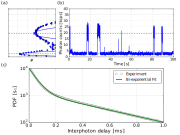
\includegraphics[width=0.95\textwidth]{02_Figure_2_transient_single_site_results}%
\caption{\textit{\textbf{Fluorescence enhancement of single Cy5 molecules with transient binding.}
(a) Binned intensity histogram (squares) with a fit with two Poisson distributions (blue lines). 
(b) Binned fluorescence time trace (bin time = $10\,\mbox{ms}$). 
From these two plots, two intensity levels are clearly recognized: the high 
level corresponds to the enhanced fluorescence signal of one Cy5 molecule at 
a fixed position in the hot spot while the low level corresponds to the 
intensity from gold nanorod luminescence plus the contribution of all diffusing molecules (enhanced and unenhanced) in the detection volume.
(c) Interphoton delay probability density function (PDF) obtained 
from the TTTR measurements (empty dots) and a bi-exponential fit, one 
for each intensity level. The retrieved intensities from this fit are 
shown in green dashed lines in (a) and (b), and coincide with the 
high and low fluorescence levels in the time trace.
\label{fg:transient_results}}}
 \end{figure}



Figure \ref{fg:transient_results} shows the experimental results
 on our two-intensity system. On panel (a), on the top left, we 
show the typical histogram of number of photons per bin time, 
characterizing the binned fluorescence time trace of panel (b), 
which shows the fluorescence time trace. The solid lines in panel (a) 
are fits with two Poisson distributions. We attribute the deviation 
from the experimental histogram to additional experimental noise not 
included in the model. Two levels can be clearly identified. The high-fluorescence 
level corresponds to hybridized docking and imaging DNA strands, so 
that a dye molecule is immobilized in the hot spot, emitting enhanced 
fluorescence. After some seconds the DNA de-hybridizes either before 
or after bleaching of the dye, and the imaging strand leaves the 
hot spot. In both cases, the signal has vanished. The low-level signal 
corresponds to the luminescence of the 
gold nanorod itself and to the background fluorescence of diffusing
and unenhanced molecules in the confocal volume. This system 
thus fulfills our purpose by providing a stream 
of detected photons with two well-defined intensity levels. 
We would like to retrieve these two levels using the interphoton 
delay distribution by fitting a bi-exponential function. 
Figure \ref{fg:transient_results} (c) shows the experimental curve 
and the fitting, from which we extracted the two intensity levels 
marked in (a) and (b) with dashed lines. These levels clearly 
reproduce the levels evidenced by the binned time trace and intensity 
histograms, but they were obtained without the need of any arbitrary 
bin time. 

The results in this simple case show how useful this type of analysis 
can be, since we were able to extract useful information from our experimental
TTTR data without introducing any arbitrary parameter.


\section{Slow diffusion in a 2D Gaussian intensity profile\label{sec:gaussian2d}}

A more realistic scenario to use our analysis is the problem of 
two-dimensional diffusion of fluorescent molecules in a Gaussian beam, 
described by an intensity function $I(\ve{r}) = I_0 \exp[-r^2/\sigma^2]$, 
where $(r,\theta)$ are the normal polar coordinates in the plane and 
$\sigma$ represents the waist of the beam.  
In this case, the intensity profile is bi-dimensional and only depends
on the distance to the center of the beam. We take a concentration 
$C$ of fluorescent molecules per unit area. Using this intensity 
distribution in Eqn. (\ref{eq:result}) we calculate the expected 
interphoton delay distribution $p_G(\tau)$and find the integral form
\begin{equation}
	p_{G}(\tau)=-\frac{\mbox{d}}{\mbox{d}\tau}
	\left[ \exp\left(-C \sigma^2 \pi \int_{\epsilon}^1\left(1-\exp\left[-\tau I_0 u \right]\right) 
	\frac{\mbox{d}u}{u}\right)    \right]\,,  
\label{eq:gaussian2d}
\end{equation}
where $\epsilon \equiv \exp\left(-\frac{R^2}{\sigma^2}\right)$ 
and $R$ is the maximum radius accessible to the diffusing molecules. Because of the smooth variation of the Gaussian beam, many single-molecule bursts have the same maximum intensity. Therefore, FCS  provides a good estimate of single-molecule brightness. The case of enhanced fluorescence discussed in Sec. V is much more difficult.

We studied the Gaussian case experimentally in a regular confocal microscope 
by confining the diffusion of ATTO647N dye molecules in a lipid bilayer, 
obtaining a two-dimensional case and a reduced diffusion coefficient of 
$D=4.4\, \upmu$m$^2$s$^{-1}$, as presented previously\cite{pradhan2016goldnanorodenhanced}. 

\begin{figure}
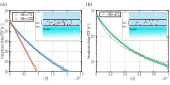
\includegraphics[width=0.99\textwidth]{03_Figure_3_2D_gaussian_with_single}%
\caption{\textit{\textbf{Two-dimensional molecular diffusion probed with a Gaussian beam.} 
(a) Interphoton delay probability density function (PDF) for the case 
of high concentrations of molecules, with an average
number of molecules $\langle N \rangle=7.5$ or $120$ in the detection area 
$A=\pi\sigma^2$ (corresponding to approximately $14$ and $225$ molecules 
per $\upmu\mbox{m}^2$, respectively). The circles are experimental values 
while the dashed lines are fits with the model from Eqn. (\ref{eq:gaussian2d}). 
(b) Interphoton delay probability density function for the case of a low concentration
of molecules, $\langle N \rangle=0.5$ (approximately $0.9$ molecules per $\upmu\mbox{m}^2$). 
In this case we find clear deviations from our model of slow diffusion, possibly indicating averaging of number fluctuations by diffusion, and a more exponential-like decay. The insets show a scheme of the experimental configuration of the lipid bi-layer on the glass surface with the typical dimensions involved (not to scale).
\label{fg:gaussian2d}}}
\end{figure}

We performed the experiment for high and low concentrations 
of molecules in the lipid bilayer and fitted 
the experimental interphoton curves with $p_{G}(\tau)$ from 
Eqn. (\ref{eq:gaussian2d}) using the experimental value for the beam 
waist, $\sigma=292$ nm. Figure \ref{fg:gaussian2d} shows the experimentally 
obtained interphoton delay probability density function for high (a) and 
low (b) concentrations along with the corresponding fits using our theoretical result. 
We note that the higher the concentration, the more the delay distribution 
resembles a single exponential. Indeed, a single exponential is expected in 
the limit of extremely high concentrations, where fluctuations $\Delta N$ 
of the number of molecules $\langle N \rangle$ in the Gaussian area become 
negligible, leading to a constant detected intensity and therefore to a single-exponential 
interphoton delay distribution.

A closer look at the curves in Fig. \ref{fg:gaussian2d} 
reveals that the case of high concentration is well captured 
with our model while the low concentration case is not. This is a direct 
consequence of the main approximation in our model, that largely neglects the 
effect of diffusion. Another phenomenon we have ignored is photobleaching of 
the molecules in the laser beam. These deviations from our model could thus be
studied through the interphoton delay distribution. 


\section{Interphoton delay distribution with fluorescence enhancement\label{sec:model_enha}}

We now turn to the case of plasmonic enhancement by an individual
nanoparticle. The spatial distribution of fluorescence enhancement by 
a plasmonic structure is complex and depends on many parameters. For 
simplicity's sake, we model this distribution as a spherically symmetric 
profile around a spherical nanoparticle. The fluorescence intensity 
profile is taken as the sum of a Gaussian confocal volume similar to 
that of the previous section, and of a near-field component modeled as 
a steeply decaying power law of radius: 
\begin{equation}
I(r) = W_0 \left[ \exp \left(-\frac{r^2}{\sigma^2} \right) + E \left(\frac{R_{NP}}{r}\right)^\alpha  \right]\,, 
\quad r \leq R_\textrm{NP}
\label{eq:enhancement_model}
\end{equation}
where $W_0$ is the unenhanced intensity, $\sigma$ the width of the Gaussian 
illumination, $E$ the maximum enhancement factor at or close to the 
particle's surface, and $R_\textrm{NP}$ the nanoparticle radius. The 
exponent $\alpha$ is a free parameter used to simulate the short-range 
variation of the near field. For pure excitation enhancement by a electrostatic 
dipole field $\alpha =6$, for combined excitation and radiative enhancements 
of an electrostatic dipole field, we would have $\alpha =12$.
We note that to recover the Gaussian case studied in the previous 
section, we need to take $R_\textrm{NP}=0$. In order to obtain 
$p(\tau)$ we insert Eqn. (\ref{eq:enhancement_model}) into Eqn.
(\ref{eq:result}) and numerically solve the integral for $R_\textrm{NP}=25$ nm. 

\begin{figure}
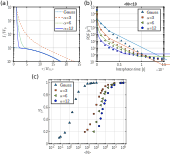
\includegraphics[width=0.95\textwidth]{04_Figure_4_enhancement_model_beta}%
\caption{\textit{\textbf{Simple model for plasmonic enhancement in two dimensions.} 
(a) Normalized radial intensity distributions for Gaussian (blue doted line), $\alpha=3$ (red dashed line),
$\alpha=6$ (green dashed line) and $\alpha=12$ (blue solid line). For all the cases the 
unenhanced intensity is $W_0=1.5\times10^4\,\mbox{cps}$ and for the enhanced case we used
$R_\textrm{NP}=25 \,\mbox{nm}$ and $E=1000$.
(b) Interphoton delay probability density function for the three cases presented in (a)
for a mean number of molecules $\langle N \rangle =10$ in the Gaussian area. The symbols present
the data from the numerical evaluation of $p(\tau)$ and the solid lines are fits with a stretched exponential. 
We intentionally reduced the density of points for display.
(c) Extracted $\beta$ from the stretched exponential fit as a function of the mean number of 
molecules in the Gaussian area. The color code is maintained throughout the whole figure. 
\label{fg:enahncement_model}}}
\end{figure}


Figure \ref{fg:enahncement_model} (a) shows the comparison 
of the spatial intensity distribution for three different 
values of the exponent $\alpha$ with the unenhanced case. 
With these intensity spatial distributions, we calculated the interphoton
delay distribution by numerically solving the integral in Eqn. (\ref{eq:result}). 
Note that the area inside the nanoparticle is not accessible 
to the molecules so the integration was carried for $r \geq R_\textrm{NP}$.
The obtained distributions are shown in Fig. \ref{fg:enahncement_model} (b) 
for the case of $\langle N \rangle=10$ molecules in the Gaussian area ($A=\pi \sigma^2$).  
Clearly the distributions with enhancement show more probability density at extremely 
short interphoton times, corresponding to the high emission rates produced by 
molecules occasionally entering the near-field area with high enhanced intensities. 
These events correspond to bright bursts in the fluorescence time trace. 
The lower the concentration of molecules, the more seldom these events will be, 
and the further away the delay distribution will be from a single exponential. 

In order to qualitatively compare the interphoton delay distributions for the 
different cases, we decided to fit them with stretched exponentials:
\begin{equation}
f(\tau) = A \exp\left[ -(\lambda \tau)^\beta\right]
\label{eq:strechted_exp}
\end{equation}
to characterize the deviation of the interphoton delay distribution from a single 
exponential. As we mentioned before, in the case of very high molecular concentration 
we expect to recover $\beta=1$, i.e. an exponential behavior, whereas large number 
fluctuations will give rise to strong deviations from single exponential and to a smaller 
stretching exponent. The empiric fit function in Eqn. (\ref{eq:strechted_exp})
works reasonably well for short times, but fails to reproduce the long-time tails of the 
delay distribution. Therefore, we focus our analysis on the short-time domain, which contains 
the most useful information about plasmonic enhancement.


We fitted the calculated probability density functions for different concentrations of molecules
ranging from a very diluted sample ($1$ molecule in the Gaussian area, $3\times10^{-3}$ 
in the near-field area) to an extremely 
high number of molecules ($10^{6}$ in the Gaussian area, $3\times10^{3}$ in the near field). 
Figure \ref{fg:enahncement_model} (c) 
shows the obtained stretching exponent $\beta$ as a function of concentration and for the Gaussian
beam and the enhanced case with three different exponents $\alpha =3$, $6$, and $12$.
In the Gaussian case we obtain an exponential behavior, 
characterized with $\beta=1$ only for $\langle N \rangle \geq 100$. This corresponds
to the situation when number fluctuations in the
detection area are negligible and thus a nearly constant detected intensity is obtained. 

To obtain a single-exponential interphoton delay distribution in the enhanced case, 
we should reach the high-density regime mentioned above, but considering the near-field area.
Since the ratio of the near-field area $A_\textrm{NF}$ (consider as the area 
that contains intensities higher than $EW_0\exp(-1)$) and the far-field area 
$A_\textrm{FF}=\pi\sigma^2$ is $\frac{A_\textrm{NF}}{A_\textrm{FF}} \sim 3\times10^{-3}$,
we roughly expect a difference of $3$ orders of magnitude in the number of molecules 
needed to reach the single-exponential limit. Indeed, this is what our
curves show, where for the enhanced case we approach $\beta=1$ around 
$\langle N \rangle=10^5$. 

From Fig. \ref{fg:enahncement_model} (c), we see that the stretching exponent steeply 
decreases with concentrations, as expected from the qualitative discussion above. 
This effect is more pronounced for a steeper decay of the fluorescence intensity 
profile, i.e., for larger values of $\alpha$. For very small concentrations, the 
stretched-exponential fit becomes poor, and the associated beta values have been 
omitted. We also note that the slope of the variation of $\beta$ with concentration 
is not very sensitive to the near-field decay characterized by $\alpha$ 
(see Fig. \ref{fg:enahncement_model} (c)). 


\section{Fluorescence time traces with enhancement by a gold nanorod \label{sec:enhancement}}

We now turn to results of an experiment with configuration similar to the one 
presented in section \ref{sec:gaussian2d}. A Gaussian beam is focused on a 
single gold nanorod immobilized on a glass substrate, and dye molecules diffuse 
in a lipid bi-layer deposited on the same substrate, similar to Ref. \cite{pradhan2016goldnanorodenhanced}. 
A fluorescence signal is produced whenever a dye molecule enters the 
diffraction-limited Gaussian beam, and an enhanced fluorescence 
signal appears if the molecule then enters either of the plasmonic hot spots 
around the tips of the gold nanorod. In order to obtain the enhancement value, 
we need to compare the detected intensity from a single-molecule enhancement event 
with the unenhanced intensity detected using the same experimental conditions, which 
was $100$ kcps\cite{pradhan2016goldnanorodenhanced}.

\begin{figure}
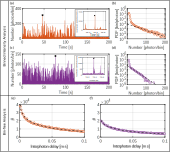
\includegraphics[width=0.95\textwidth]{05_Figure_5_enhancement_traces}%
\caption{\textit{\textbf{Single-molecule fluorescence enhancement by gold nanorods.} 
The top panel shows the typical binned-intensity plots while the bottom 
panel shows the bin-free interphoton histograms.
(a),(c) $1$ms-binned fluorescence intensity as a function 
of time for two individual nanorods. The nanorod in (a) presents
a higher enhancement factor. The black cross in the plot indicates the 
maximum recorded intensity. The insets show respective zooms around the maximum
intensity bursts.
(b),(d) Burst intensity histograms showing number of photons per $1$ms-time bin for the traces in (a) and (c), 
respectively. The dashed black lines are exponential fits to the tail of the distributions. 
(e),(f) Interphoton delay probability distributions for the experimental traces 
shown above. We also show a fit to the curves using a stretched-exponential model.
The curves in purple (orange) correspond to traces (a) and (c) respectively and this color code is maintained throughout the whole figure. 
\label{fg:GNRS}}}
\end{figure}
% left in comment what michel wrote
%- brief description of time trace (see Ref. \cite{pradhan2016goldnanorodenhanced}) with long weak bursts corresponding to far field and occasionally intense but short bursts corresponding to diffusion in the near field. For the traces shown, the selection of the highest burst(s) lead to enhancement factors of XXX.

Figure \ref{fg:GNRS} presents the TTRR experimental data obtained in 
such an experiment in different ways, for two different gold nanorods. 
In the top panel we have the bin-dependent time traces and burst histograms (binning time $1$ ms) while the lower panel
shows the ``bin-free'' interphoton delay histograms.
If we analyze the binned time traces in Fig. \ref{fg:GNRS} (a) and (c) and the insets, we observe that they
present a qualitatively similar behavior: there is a constant baseline
intensity, long weak bursts corresponding to molecules exploring the far field area and occasionally 
intense but short bursts corresponding to diffusion in the near-field area\cite{pradhan2016goldnanorodenhanced}. 
The black crosses in the time traces indicate the highest burst found in that trace, which leads to 
``cherry picking'' enhancements factors $E^{(CP)}=(4.5 \pm 1.5)$ and $E^{(CP)}=(2.3\pm 0.7)$.

%- characterization of time trace by histogram of binned data; comparison of histograms for two types of nanorods, one with weak enhancement, the other with stronger enhancement. Discuss the histograms and the decay of probability with number of photons per bin. Physical interpretation: unlikely to have strong bursts because the molecule has to come very close to the nanorod tip, probability decays as distance in 2D, square of distance in 3D.

%- Should give a power law, but experimentally resembles more an exponential cutoff. Possible reasons for that deviation: photobleaching, detector limitations, possibly role of diffusion during the measurement of the burst.

Another useful way to characterize the experimental enhancement is the histogram 
of binned intensities, as shown in Fig. \ref{fg:GNRS} 
(b) and (d). These histograms show a rapidly-decaying tail where the characteristic 
decay intensity is larger for the top nanorod, indicating stronger enhancement. The 
steep decay of these histograms can be qualitatively understood by recalling the spatial 
distribution of near-field intensity at resonance, which is
extremely high (around $300$ times the incident intensity) very close to the tips and 
decays rapidly with distance to the tips. 
Therefore, there is a low probability for a diffusing molecule to reach this small area. 
For small distances, this probability density goes linearly with distance 
in the bi-dimensional case, and as the squared distance in three-dimensional case. 

We analyzed the intensity distribution around a rod ($25\times47$ nm$^2$), calculated 
from a discrete-dipole approximation \cite{khatua2014resonant}. In the 2D case, we found an 
approximate power law distribution with exponent $1.37$. However, the tail of the 
experimental distribution is exponential, as can be seen in Fig. \ref{fg:GNRS} (b) and  Fig. (d).
There are several possible sources for such a discrepancy, such as the effect of photobleaching,
the dead time of the detectors, and possibly the role of diffusion during the burst.
Confirming the role of each of these effects would require full numerical calculations, with 
an accurate description of these effects. However, this is a complex and computationally 
extensive problem that is out of the scope of this paper.

%- Whatever the reason for this deviation, we may estimate the maximum enhancement through the histogram. Notice that stronger enhancement corresponds to a broader histogram, with cutoff for larger number of photons. If we model the histogram decay as a single exponential $P(N)=\exp(-N/N_0)$, we can estimate the maximum number of photons in the strongest burst as $N_0 \ln(M)$, where $M$ is the total number of attempts and is proportional to the duration of the trace. For a typical value of M=$10,000$, we find 9.2 $N_0$ (check this with the ratio of time trace to burst duration...).

Regardless of the reason for this deviation, we may empirically estimate
the maximum enhancement through the histogram. Note that stronger enhancement 
corresponds to a broader histogram, with cutoff for larger photon number.
If we model the tail of the normalized histogram decay as a single exponential $P(N)=M\exp(-N/N_0)$, 
we can estimate the maximum number of photons in the strongest burst by solving 
$P(N_c)=\varepsilon$ with $\varepsilon=1/N_{\mbox{bins}}$, where $N_{\mbox{bins}}$ is 
the total number of bins in the time trace, here about $10^6$. This estimate roughly 
corresponds to a probability equal to unity of observing such an intense burst in the 
time trace. We thus obtain $N_c = N_0 \ln(M/\varepsilon)$. For a typical value of 
$M\sim\times10^{-3}$, we find $6.9 N_0$. With this method we obtain $E^{(H)}=(4.9 \pm 0.2)$ 
and $E^{(H)}=(2.40 \pm 0.05)$ for the plotted data in Fig. \ref{fg:GNRS} (b) and (d).

%- We can also estimate the enhancement factor from the maximal intensity read from the histogram of delays between consecutive photons. These histograms are shown for two rods in Fig XXX. Deviations from single-exponentials are clearly seen. To characterize them, we fit the histograms with a stretched exponential of time $p(\tau)=A \exp(-(w\tau)^\beta)$, as this fit involved only three parameters, against four for a bi-exponential decay. The maximum intensity is deduced from the slope of the histogram at the shorter possible time and provides another estimate of the enhancement factor based on a statistical quantity. Fig XXX shows that larger enhancements correspond to a larger deviation of the histogram from a single exponential, and to a larger slope at the smallest bin time of the histogram. 

We can also estimate the enhancement factor from the interphoton delay histograms. These histograms are shown for the same
two nanorods in Fig. \ref{fg:GNRS} (e) and (f). 
Deviations from single-exponentials are clearly seen. To characterize them, we fit the histograms 
with a stretched exponential of time (see Eqn. (\ref{eq:strechted_exp})), which involves only 
three parameters, against four for a bi-exponential decay. The maximum enhanced intensity is deduced from 
the slope of the histogram at the shorter measured interphoton time ($200$ns) and provides another estimate of the 
enhancement factor based on a statistical quantity. Figures \ref{fg:GNRS} (e) and (f) 
show that larger enhancements correspond to a larger deviation of the histogram from a 
single exponential, and to a larger slope at the smallest bin time of the histogram. With 
this procedure, we obtained an enhancement value of $E^{(I)}=(4.3 \pm 0.2)$ and 
$E^{(I)}=(2.0\pm 0.1)$ for the presented nanorods.

%\subsection{Comparison of the estimates of enhancement factors by the 3 methods}

We now compare the maximum intensities and the associated enhancement factors obtained 
for five different nanorods, for the whole $200$ s-long time trace, and after splitting each trace into 5 sub-traces 
of $40$ s each. Figure \ref{fg:en_cor} shows the example of the binned time trace (a),
burst histogram (b) and the interphoton delay histogram (c) for the whole trace and for each sub-trace. 

The associated results for the different methods are correlated in Fig. \ref{fg:en_cor} (c) and (d).
The different symbols correspond to different nanorods and the colors refer to the different sub-traces for each rod. 
In Fig. \ref{fg:en_cor} (d) we observe an excellent correlation between the cherry-picking method and the
statistical method based on the burst intensity histograms. Note that the same symbols are clustered together,
showing that the enhancement factor obtained using different sub-traces with both methods lead to similar results.
We also correlated the results from the interphoton delay distribution with the burst intensity histograms in 
Fig. \ref{fg:en_cor} (e), where a satisfactory correlation is found and the obtained enhancement factors
are consistent with both other methods. However, the enhancement factors deduced from interphoton delay distributions present more dispersion than the other two. 

   

\begin{figure}
\includegraphics[width=0.99\textwidth]{06_Figure_6_enhancement_correlation}%
\caption{\textit{\textbf{Comparison of the enhancement factors obtained with different methods.} 
(a) Binned time traces split into five different sub-traces of $40$ s each (binning time $100$ $\upmu$s). 
The crosses show the maximum number of counts per bin obtained in each sub-trace, 
used to calculate the ``cherry-picking'' enhancement factor $E^{(CP)}$. At the top we show the 
length of the sub-traces and assign a number for reference.
(b) Normalized burst histogram in number of photons per bin obtained for each of the sub-traces presented in (a).  
We also show in dashed lines the exponential fits to the tail of the probability density. The burst histogram for the total trace is plotted as well.
(c) Interphoton delay distributions for the sub-traces and the total trace with their stretched-exponential fits. 
(d) and (e) show scatter plots of enhancement factors $E^{(CP)}$, $E^{(H)}$, $E^{(I)}$ deduced by the three methods. The different
symbols correspond to different nanorods and the colors refer to the sub-traces used to obtain the enhancement factor.
In black we show the results for the total trace. 
(d) Correlation between $E^{(CP)}$ from cherry picking and $E^{(H)}$ from burst histogram, showing an excellent correlation with slope equal to unity (dashed black line).
(e) Correlation between $E^{(I)}$ from interphoton delay histograms and $E^{(H)}$ (the dotted line is a linear fit with
slope $1$). Here, we observe more dispersion of the data.
}
\label{fg:en_cor}}
\end{figure}

%
%Fig(XXX) confirms that the three measures of the enhancement factor are consistent with one another. Check that more spread from cherry-picking? Has to be written once the results are available...

Figure \ref{fg:en_cor} confirms that the estimates of the enhancement factor deduced by three very different methods (time trace, burst histogram, interphoton delays) are similar in value and consistent with one another. The values deduced from the cherry-picking procedure are surprisingly stable and reliable. They agree well with extrapolations of burst histograms fitted with a single-exponential function, although the justification for this analytical form is still missing. Unexpectedly, the enhancement factor deduced from the interphoton histogram appears to be the most sensitive to statistical fluctuations. This can be a consequence of fitting with a stretched exponential, which is an approximation. However, this method has the unique advantage that it can be applied to the experimental data directly, without any need for binning or other arbitrary parameters.


\section{Conclusions}

In this paper we characterized single-molecule fluorescence traces 
obtained with a time-tagged time-resolved setup in a variety of 
experimental conditions with the \textit{interphoton
delay distribution}. This avoids the introduction of an arbitrary binning time. 

We presented a theoretical treatment for the case of nearly static, slowly diffusing molecules that
relates the interphoton delay distribution to the spatial intensity 
distribution explored by the molecules. With this model, we could reproduce the simple case of 
switching between two states with different intensities. We also explored the problem of molecules diffusing in two dimensions in a Gaussian beam. Our nearly static model works well at high concentrations, but shows deviations at lower concentrations, which may arise from diffusion or from other experimental deviations from the model.

Furthermore, we used the interphoton delay distribution to measure the 
fluorescence enhancement factor by individual gold nanorods. For our experimental traces with moderate enhancements, we obtained
enhancement factors that are consistent with the accepted methods in the 
community with the advantage of avoiding the introduction of any arbitrary
parameter that may influence the results. 
In the future, we plan to perform similar comparisons for the very 
large enhancement factors obtained with weakly emitting dyes.
%=========== Supporting info ========
% \newpage
% \section{Supporting Info}
\graphicspath{{./chapters/c3_binfree/si_figure/}}

\section*{Transient Binding sample preparation}


\section*{Binned time traces dependence with bin time}



\section*{Lipid bilayer sample preparation}



\section*{2D Numerical simulations}

The current program is organized in only one script, simualtion2d.m and contains several subroutines. It also uses the program generate\_simulation\_parameters.m to set all the needed parameters for the simulation. These are divided in two sets, the physical parameters and the simulation parameters. 
The former set of parameters corresponds to the experimentally relevant variables while the latter corresponds to the extra parameters needed to run the simulation and are not related to the experimental conditions but need to be selected to run the simulation. 
The output of the program is a structure that has contains the unbinned time traces, binned time traces and interphoton histograms. The physical inputs are the following: concentration of molecules $C$, intensity distribution of the incoming beam $I(\ve{r})$ and dark counts of the detector $Dc$. 
For a complete list of the simulation parameters, refer to the appendix \ref{ap:sim_param}.

The calculation consists of several steps that will be summarized in the following. 
The spatial intensity distribution input has to be a matrix $M$ with the spatial intensity distribution of the incoming beam $I(\ve{r})$ (in cps). 
The first step is done by the subroutine \texttt{calculate\_times} to simulate the absolute arrival photon times for each intensity value of the matrix 
\footnote{This can be improved in speed by not calculating the repeated intensity values more than one time and by saving the output structure in a file and loading it later instead of recalculating it.} 
within the time of the experiment, $T_{\mbox{Max}}$. This traces correspond to a single molecule placed in each pixel of the intensity matrix.
To generate the correct exponential distribution for a given intensity $I$, I use the fact that the interphoton times should follow an exponential distribution:
\begin{equation}
\Delta t_{i} = -\frac{\log\left(\zeta_i \right)}{I} \, ,
\label{eq:interphoton_simulation}
\end{equation}
where $\Delta t_{i}$ ($i=0,...,N$) represents the time between successive photons detection and $\zeta_i$ is a random number in the interval $(0,1)$. 
This way of generating the interphoton times ensures the required exponential distribution. Then by performing the cumulative sum over the interphoton times the absolute arrival times of the simulated stream of photons can be calculated for each intensity value in the input intensity matrix $M$. This data is contained in a structure named \texttt{abs\_times}. 

The next step is to calculate the number of molecules present in the simulation volume  $V_{sim}$. For a given concentration, the number of molecules contributing to the simulation is random variable that follows Poisson distribution with a mean value $\left<N_{molecules}\right> = C V_{sim}$. Since our calculation is based on the calculation of the interphoton arrival time for a fixed number of molecules $N_{molecules}$ in the simulation volume, we calculate the number of molecules needed to contain 99\% of the cases. Then, for each $N_{molecules}$ we generate the interphoton histogram as follows. We generate random positions for all the available molecules in the simulation volume and we retrieve the corresponding absolute photon arrival times from the variable abs\_times. We concatenate all this arrival time and also include extra photon detections generated by the dark counts of the detector. The mean number of dark photons in the simulation time is $Dc T_{\mbox{max}}$ and follows a poisson distribution. We use a poissonian number generator to simulate the number of detected photons in each run and then distribute them uniformly in the time trace. All this concatenated absolute photon detection times are then sorted and saved in a vector $t$. Then the histogram of the interphoton times for this vector is computed, using pre-fixed bins (with a certain number of points $Hist_{\mbox{Npts}}$) . The normalized (to the total counts) histogram is stored into the first component of a matrix of histogram counts $H$. Then we repeat this procedure $N_{\mbox{config}}$ time, using each time a new set of random positions for all the molecules, creating the matrix of dimensions $Hist_{\mbox{Npts}} \times N_{\mbox{config}}$. Then we average the normalized histograms corresponding to different spatial configurations, contained in $H$ to obtain a single histogram corresponding for a single number of molecules in the simulation volume. The final step is to perform a weighted average of the histograms for each number of molecules contributing to the simulation for a fixed concentration using the corresponding poissonian weight.



\section*{Slow diffusion case}

We simulated the case of a molecule 


\section*{Simulation Parameters\label{ap:sim_param}}

\section*{code validation\label{ap:code}}

In order to validate the simulation code we tested the results with a simple beam shape that provides an analytical solution. 
We work in two dimensions just for simplicity with a rectangular beam shape with constant intensity and zero intensity outside, described mathematically as:
\begin{equation}
I(x,y) = I_0\theta(|x-\frac{x_0}{2}|)\theta(|y-\frac{y_0}{2}|)\, ,
\label{eq:theta_intensity}
\end{equation}
with $I_0$ the maximum intensity and $x_0,y_0$ the size in lateral directions and $\theta(\zeta)$ the step function. Thus, the illuminated area has a volume of $V_0=x_0y_0$. 
For such a beam shape the interphoton probability distribution can be obtained by simple integration of equation \ref{eq:result} replacing the beam shape $I(\ve{r})$ with equation \ref{eq:theta_intensity}, obtaining
\begin{equation}
p(\tau) = I_0 C V_0 \exp[-\tau I_0-C V_0(1-\exp(-\tau I_0))]\,.
\label{eq:theta_interphoton_distribution}
\end{equation}

Figure \ref{fg:square_beam}(a) shows an example in a particular case when the dimensions are the same for the two directions and \ref{fg:square_beam}(b) shows plots for the analytical solution for different intensities and concentrations.




 \begin{figure}
 \centering
 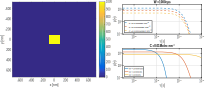
\includegraphics[width=\textwidth]{square_illumination}%
 \caption{\textbf{Simple illumination profile that provides an analytical solution to test the simulation code} 
(a) Colormap plot of the square-shaped beam we use for validating the code. We used $x_0=y_0=182$ nm and $I_0=1000$ cps.
(b)Analytical plots of the interphoton probability distribution for different intensities and concentrations. 
\label{fg:square_beam}}
 \end{figure}


%\figdouble{square_illumination}{square_illumination_analytical}{fg:square_beam}{Simple illumination profile that provides an analytical solution to test the simulation code}{ \figa Colormap plot of the square-shaped beam we use for validating the code. We used $x_0=y_0=182$ nm and $I_0=1000$ cps. \figb }


In order to test the code we performed simulations using this illumination distribution and compared it with the analytical result. We started with a fixed superficial concentration  C=$2 \times 10^{-4}$ molecules nm$^2$ to have a relative fast run and we changed the different parameters of the simulation, such as the number of spatial configurations to average and the total simulation time $T_{\mbox{max}}$. The comparison with the analytical curves can be seen in figure \ref{fg:sim_test}. In both cases the simulation agrees well with the analytical result and for longer simulation time or higher number of configurations, the error becomes smaller.


 \begin{figure}
 \centering
 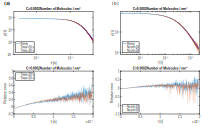
\includegraphics[width=\textwidth]{Theta_results}%
 \caption{\textbf{Test of simulation parameters and code validation} 
(a) Different total simulation times. Top: simulated and analytical curves. Bottom: relative error in the simulation.
(b) Different number of averaged spatial configurations. Top: simulated and analytical curves for different total simulation times $T_{\mbox{max}}$. Bottom: relative error in the simulation.
\label{fg:Theta_results}}
 \end{figure}


The next step was to test the simulation for different physical parameters such as the concentration of molecules and the intensity in the beam. The results for three different concentrations and intensities can be found in figure \ref{fg:phy_test}. The results again agree with the analytical curves and it can be noted that the larger the number of photons generated in the simulation the better correspondence with the analytical result.


 \begin{figure}
 \centering
 \includegraphics[width=\textwidth]{Theta_physical_test}%
 \caption{\textbf{Test of physical parameters and code validation} 
(a) Different concentrations. Top: simulated and analytical curves. Bottom: relative error in the simulation.
(b) Different intensities. Top: simulated and analytical curves. Bottom: relative error in the simulation.
\label{fg:Theta_physical_test}}
 \end{figure}
% \references{chapters/c3_binfree/biblio}